\chapter{Business Case und Ausblick}
\label{business_case}

In Wirtschaft, Wissenschaft und Verwaltung existieren verschiedenen Methoden wie Gruppen gebildet werden können, bspw. nach dem Zufall, Interessen oder persönlichen Merkmalen wie das Geburtsmonat oder ähnlichem. Ausserdem existieren bereits eine Vielzahl von Softwareanwendungen, die Organisation der Prozesse innerhalb eine Gruppe unterstützen. Als Beispiele können hier verschiedene Angebote Kollaborationssoftwareanwendungen im Unternehmenskontext oder auch Facebook, Google+ oder WhatsApp im privaten Bereich. Den Autoren ist jedoch keine Anwendung bekannt die ihren Fokus auf die schnelle und einfache Bildung von Gruppen in Echtzeit legt, ein Doodle für die Gruppenfindung. 
\newline\newline
Auch wenn der Schwerpunkt des "`Groupfindr"' nicht auf die Unterstützung der Gruppenprozesse liegt, wurden dennoch verschiedene soziale Plattformen mit dem "`Groupfindr"' mit Hilfe eines Magic Quadrant nach der Gartner Group \citet{magic_quadrant} verglichen, siehe Abbildung \ref{magic_quadrant}.  Die Merkmale die für die Einordnung herangezogen wurden sind \citet{gruppen-bildung} entnommen und durch die subjektive Einschätzung der Autoren ergänzt worden.

\begin{figure}[h]
\centering
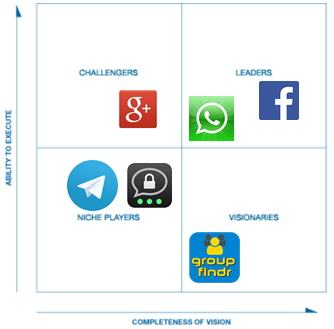
\includegraphics{graphiken/magic_quadrant.png}%
\caption{Einordnung und Vergleich des Groupfindr mit Mitbewerbern (Quelle: Eigene Darstellung)}%
\label{magic_quadrant}%
\end{figure}

Nach der Meinung der Autoren ist die "`Groupfindr"' Anwendung im Bereich der Visionären einzuordnen, da das Hauptaugenmerk auf Funktionalitäten liegt die durch die Mitbewerben nicht berücksichtigt wird. Allerdings ist der Funktionsumfang im Hinblick auf die Organisation und Kommunikation innerhalb der Gruppe nur sehr eingeschränkt.
\newline\newline
Eine Vermarktung des "`Groupfindr"' mit zwei grundsätzliche verschiedenen Lizenzmodellen denkbar. In einer ersten Varianten wird eine OnDemand oder Cloudlösung angeboten, die jeder kostenfrei nutzen kann. Eine Finanzierung könnte hierbei über Werbung erfolgen. Ausserdem wäre auch die Erweiterung um Benutzerprofile denkbar. Es ist ebenfalls denkbar für verschiedene Bildungsinstitutionen wie Universitäten oder Schulen eine werbefreie Version der Cloudlösung gegen eine Lizenzgebühr anzubieten, die dann auch an spezifische Bedürfnisse angepasst werden könnte. Die zweite Variante wäre, dass die komplette Anwendung von den Käufern selbstständig betrieben wird (On Premise Variante). Dies könnte insbesondere für Karrierenetzwerke wie XING oder LinkedIn interessant sein, um die Bildung von Projektteams für bereits auf den Plattformen ausgeschriebenen Projekten zu vereinfachen, ohne die Daten der Profile der eigenen Plattformen weitergeben zu müssen. Auch hier wäre dennoch eine Lizenzgebühr oder ggf. auch ein einmaliger Kaufpreis denkbar.
\newline\newline
Mit der jetzigen Version der Anwendung "`Groupfindr"' konnte das Problem der einfache und schnelle Gruppenbildung in Echtzeit gelöst werden. Auch wenn der momentan der Schwerpunkt auf die Gruppebildung im Rahmen von Vorlesungen im Hochschulstudium liegt, ist ein Ausbau und kommerzielle Vermarktung aus Sicht der Autoren sinnvoll und machbar.
